\section{Database storage}
\label{sec:database}
The database logical scheme has conceptually two major parts: (a.) data management
information and (b.) the attribute data. The  data management part has 4 categories:
{\em ITEM}, {\em RAW}, {\em POTREE} and {\em OSG} and the attribute data are represented
in category {\em ATTRIBUTE}.
 
Figure \ref{fig:db_erdb} contains the Entity-Relationship diagram (ERD) of the
\textit{viaappiadb}. In the coming sections each category is described briefly and
illustrated. The direct connections between each category is also illustrated.

Note that some of the nodes of the relationships are \textit{0:n} or
\textit{0:1} (with black points) instead of the usual \textit{1:n} or
\textit{1:1}. This is to illustrate that some sites and objects may have
entries in some tables but not in others. For example it is possible to have a
site in the item table which has no entry in the attributes table (tbl1\_site).

\begin{figure}[H]
\centering
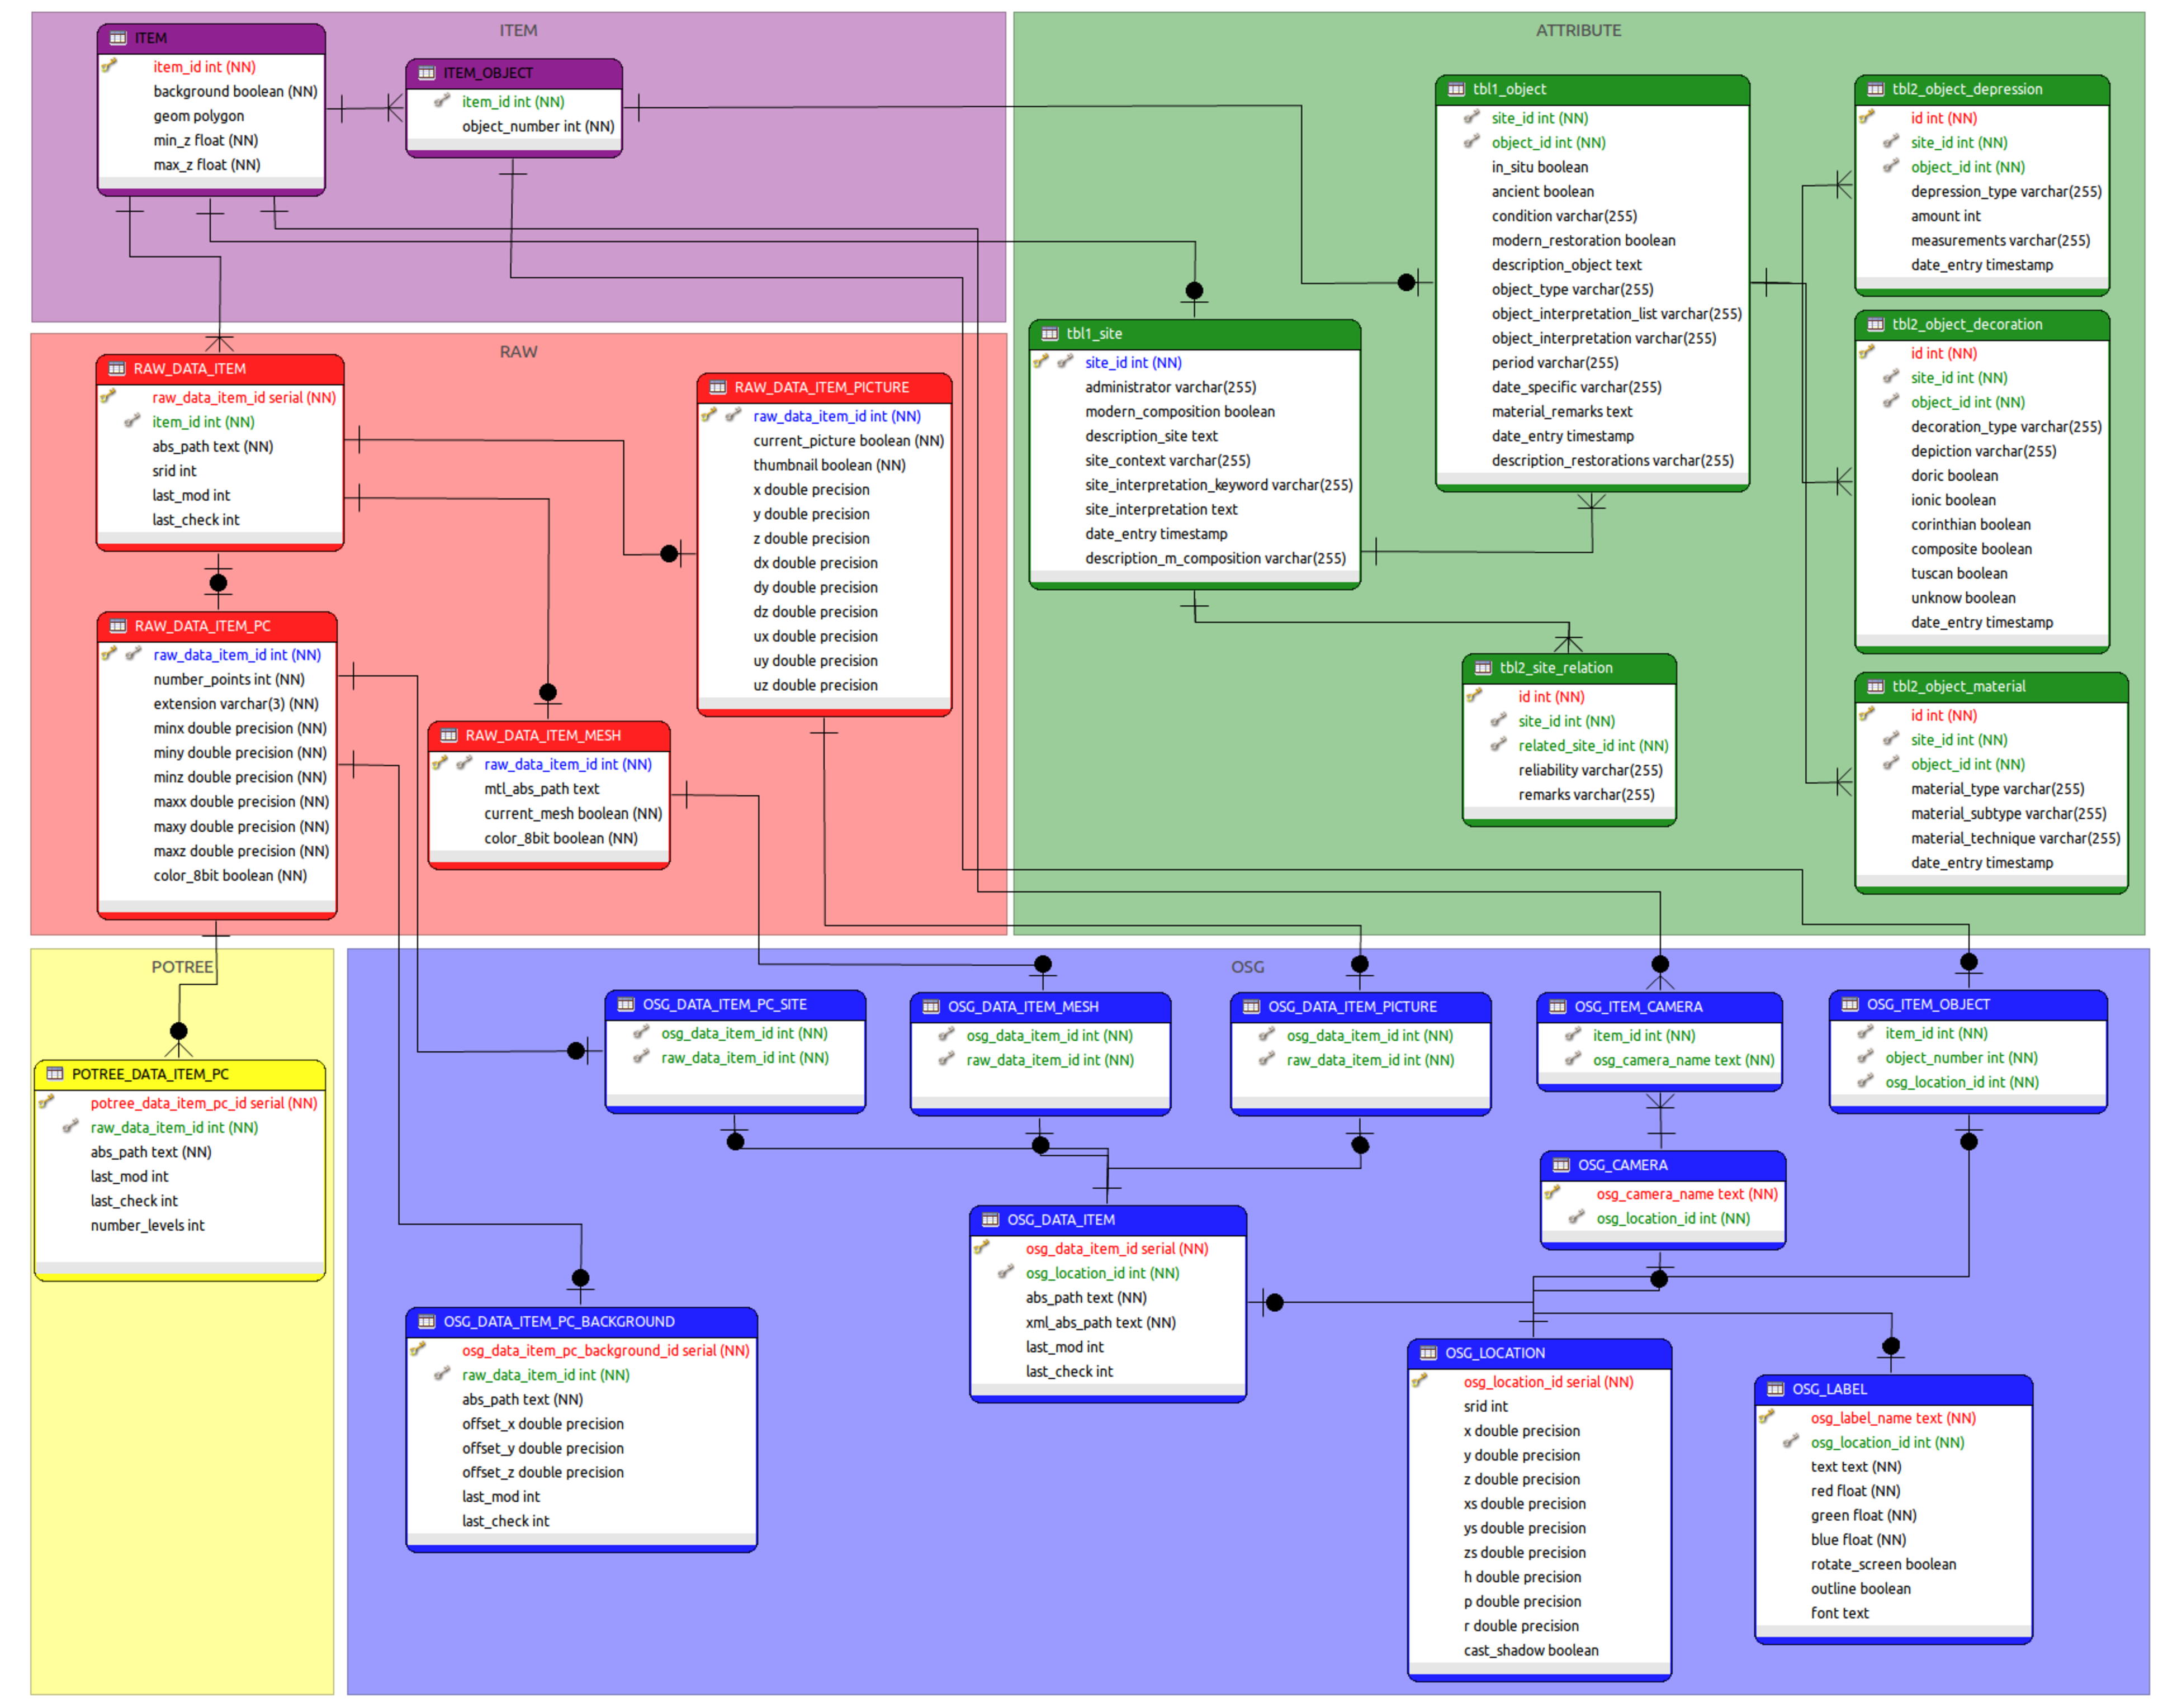
\includegraphics[scale=0.25]{fig/database/ERDB.pdf}
\caption{Entity-Relationship diagram of the \textit{viaappiadb} database with
its five categories.}
\label{fig:db_erdb}
\end{figure}

\subsection{Database logical schema categorization}
In this section describes each category and on each category the tables to store raw
data, converted data, visualization-related data and the footprints (geometries) of
the sites are located.

\subsubsection{ITEM}
Conceptually {\em ITEM} is a category containing an information about an {\em item}.
Item is any entity of interest- background (then the logical field {\em background} is
set to true (1)) or site (0). If the item of interest is an archaeological site (monument)
it contains one or more objects (parts of the site) which is reflected by the field
{\em object\_numer}. 

Figure \ref{fig:db_erdb_item} shows the relationship of the {\em ITEM} category with
the other categories. The {\em ITEM} category is on the top of the categories' hierarchy.

\begin{figure}[H]
\centering
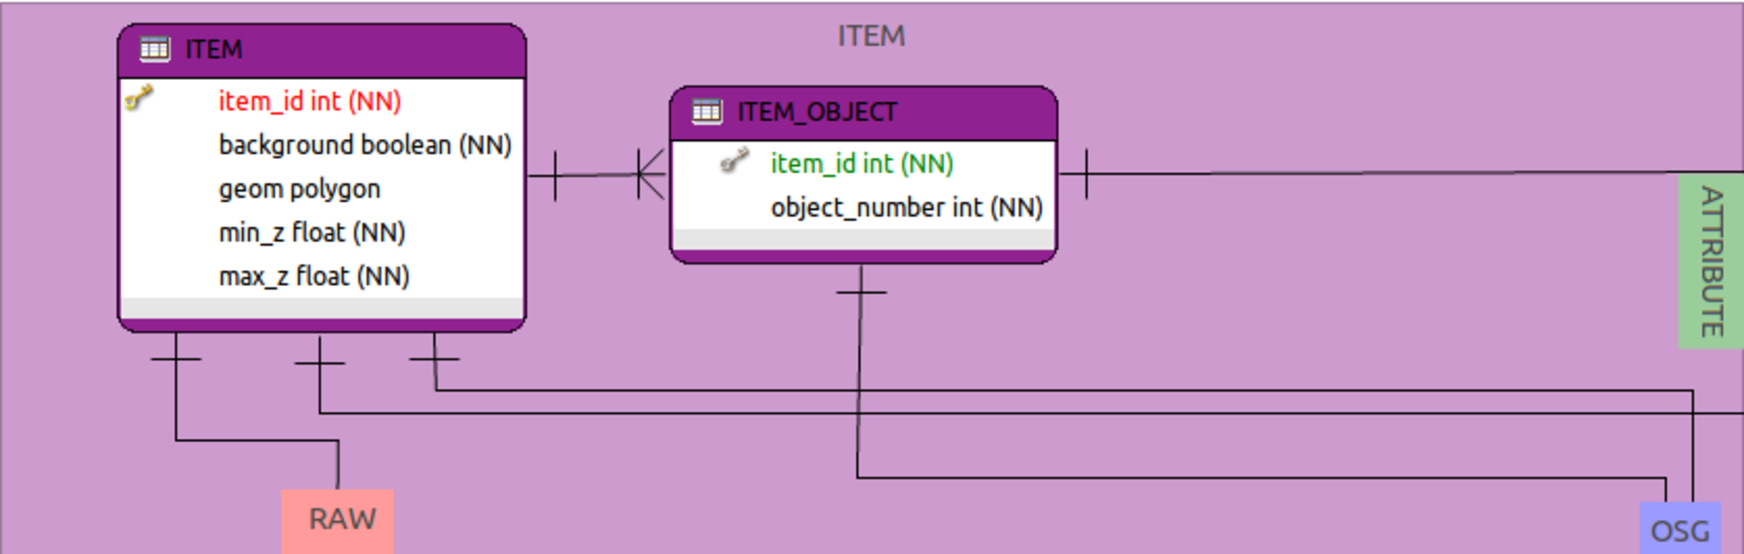
\includegraphics[scale=0.35]{fig/database/ERDB_ITEM_conn.pdf}
\caption{Entity-Relationship diagram of category ITEM and indicated connections
with other categories.}
\label{fig:db_erdb_item}
\end{figure}

\subsubsection{RAW}
The {\em RAW} category contains all the \textit{raw data} gathered for given item.
The most important meta-data is the location in the Data structure (Section~\ref{sec:data_structure}),
stored in the {\em abs\_path} field. These data can be either point clouds (PC),
meshes (MESH) or pictures (PICTURE). Each of these types is represented by a separate
table with the specific for that data type properties. The {\em RAW} category is
related to the derived data categories {\em OSG} and {\em POTREE} as indicated on
Figure~\ref{fig:db_erdb_raw}.

\begin{figure}[H]
\centering
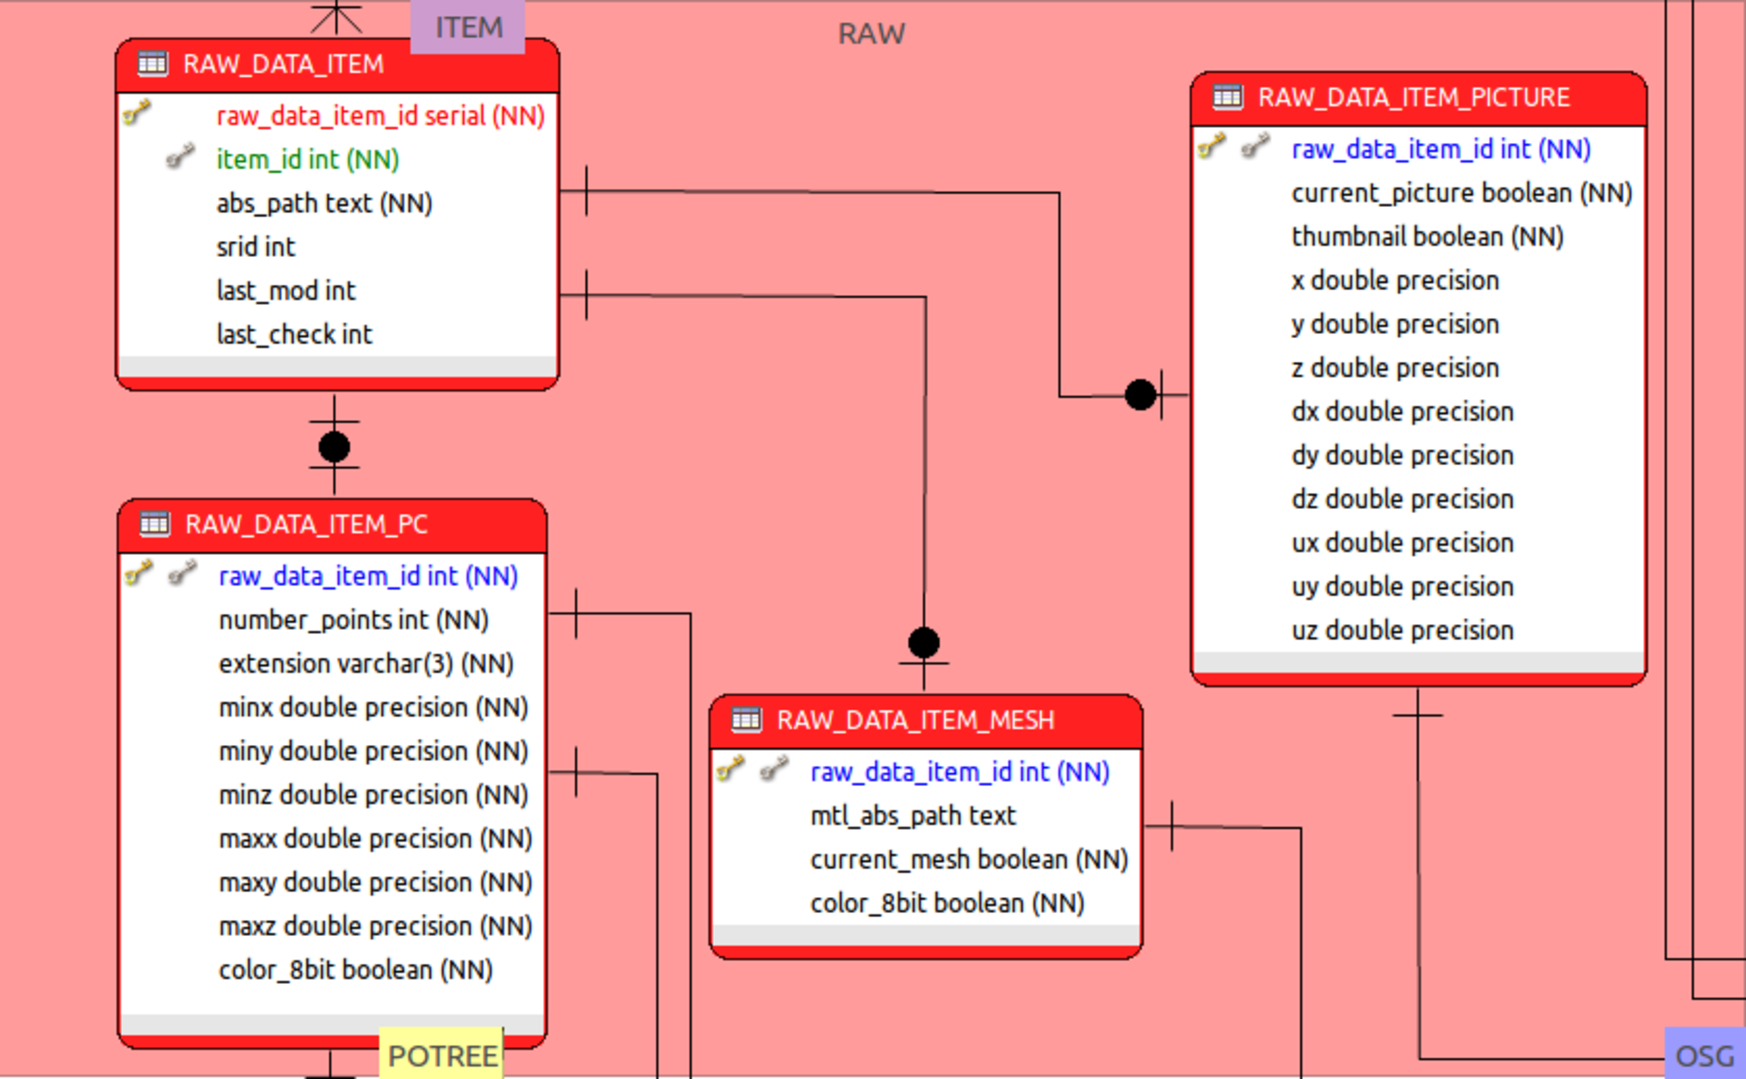
\includegraphics[scale=0.35]{fig/database/ERDB_RAW_conn.pdf}
\caption{Entity-Relationship diagram of category {\em RAW} and indicated connections
with other categories.}
\label{fig:db_erdb_raw}
\end{figure}

\subsubsection{OSG}
The {\em OSG} category represents the OSG \textit{converted data} used for the
desktop based viewer. Figure \ref{fig:db_erdb_osg} it is related to the RAW data
(from where it is derived) and to the ITEM category. The tables in this category
reflect the possible data types: PC, meshes and pictures. Most importantly, this
category contains information needed for the \textit{visualization}, like specifics
of the background and items, the camera, location (bounding box) and label. 

\begin{figure}[H]
\centering
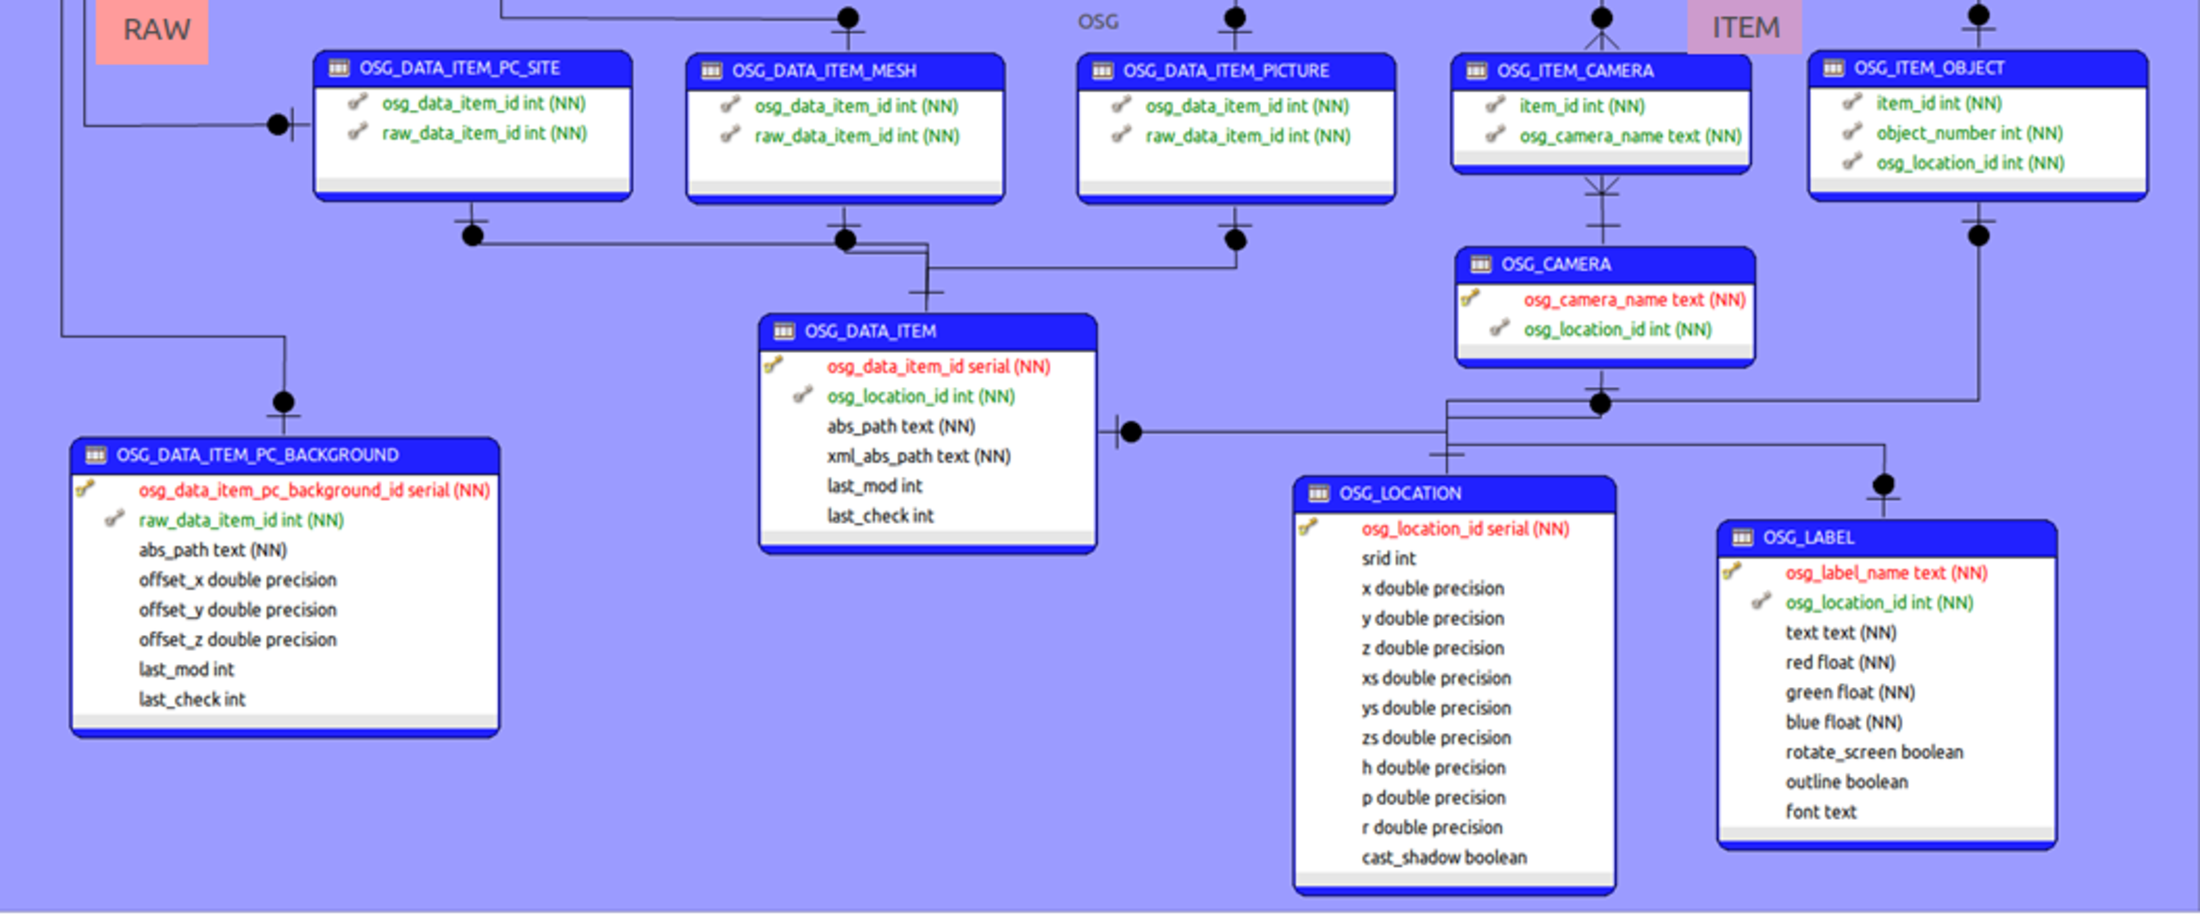
\includegraphics[scale=0.35]{fig/database/ERDB_OSG_conn.pdf}
\caption{Entity-Relationship diagram of category {\em OSG} and indicated connections
with other categories.}
\label{fig:db_erdb_osg}
\end{figure}

\subsubsection{POTREE}
The {\em POTREE} category is illustrated on Figure \ref{fig:db_erdb_potree}. It
is related only to the {\em RAW} category from which it is derived using the Potree
converter and stores only data of the PC type and conversion parameters ({\em number\_levels}).

\begin{figure}[!H]
\centering
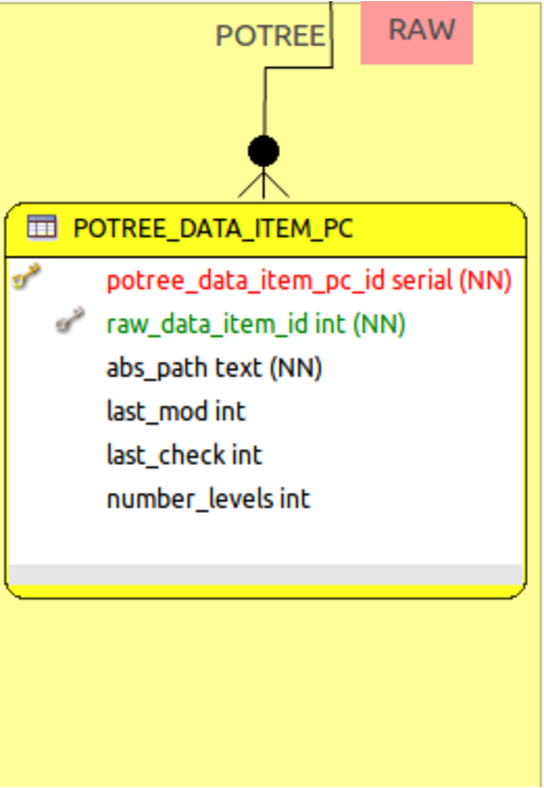
\includegraphics[scale=0.35]{fig/database/ERDB_POTREE_conn.pdf}
\caption{Entity-Relationship diagram of category {\em POTREE} and indicated
connections with other categories.}
\label{fig:db_erdb_potree}
\end{figure}

\subsection{Attribute data}
The attribute part of the DB is represented only by one category, {\em ATTRIBUTE}
(Figure \ref{fig:db_erdb_attribute}). It is connected only to the {\em ITEM} category.
These are the meta-data collected during the field work and are primarily of research
interest to the archaeologists as it contains all domain-related data enabling browsing
and filtering of sub-parts of the data of interest.

\begin{figure}[H]
\centering
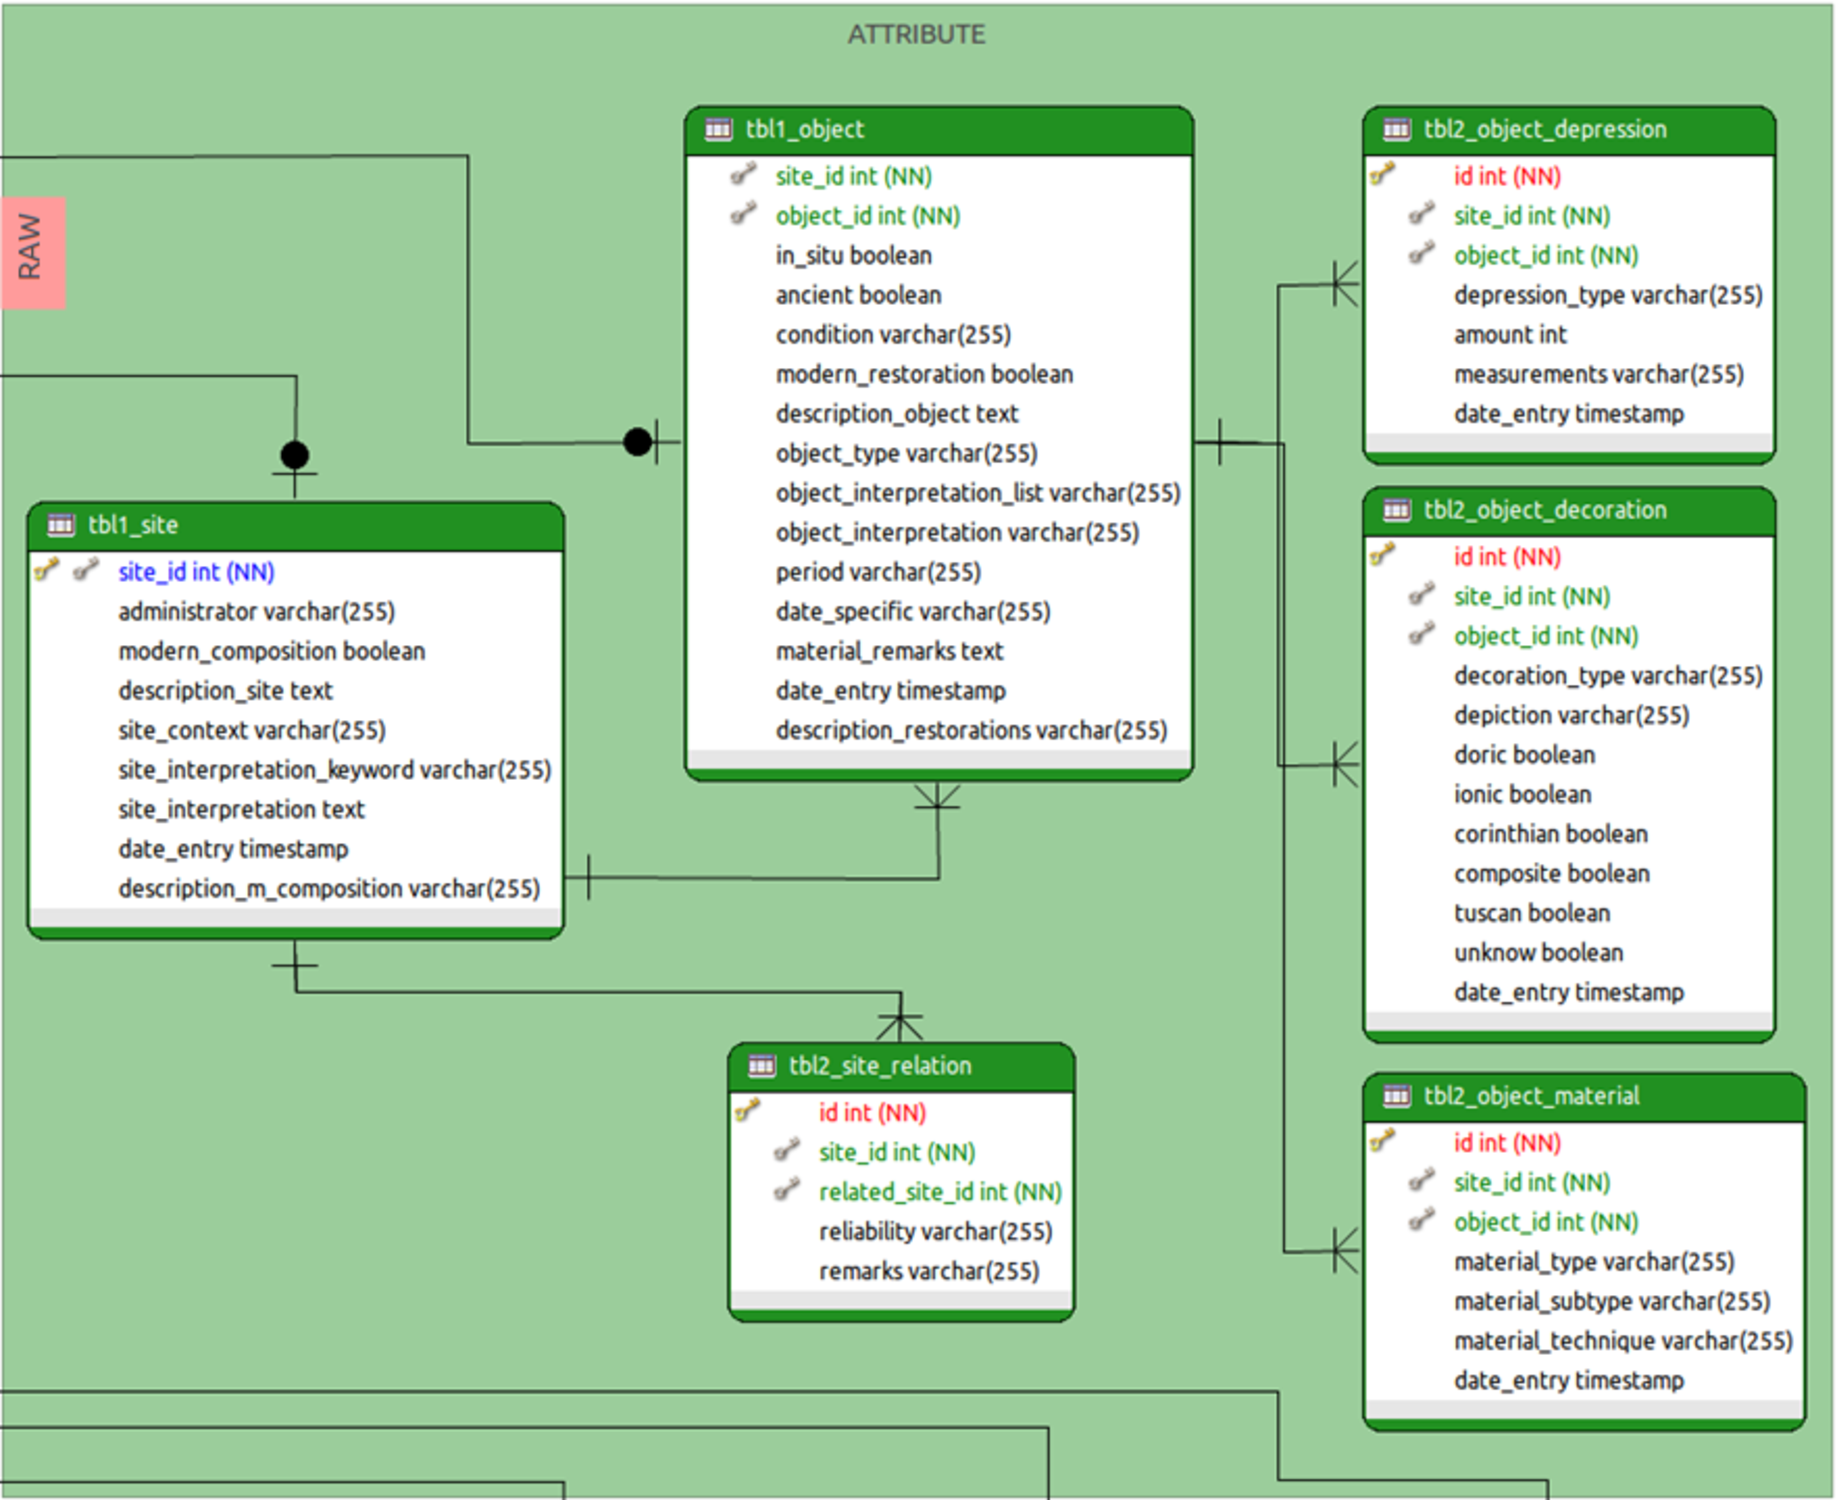
\includegraphics[scale=0.35]{fig/database/ERDB_ATTRIBUTE_conn.pdf}
\caption{Entity-Relationship diagram of category {\em ATTRIBUTE} and indicated
connections with other categories.}
\label{fig:db_erdb_attribute}
\end{figure}

The \textit{viaappiadb} database is running in the Via Appia Linux server. See
Section~\ref{sec:software} on how to get an account in the database.

